%%%%%%%%%% NO OLVIDAR COLOCAR ESTE COMENTARIO CON EL NUMERO DE EJERCICIO %%%%%%%%%%%%%
%%%%%%%%%%%%%%%%%%% EJERCICIO 2 %%%%%%
%%Text bf para negrilla , el \\ es para el salto de linea.
%%El primer \\ hace un espacio en el texto y el 2 \\ crea otro espacio
\textbf{Ejemplo 2}\newline
El jefe de producción de una fábrica debe decidir entre dos máquinas A y B. Las características de cada una son: \\
\begin{center}
		\begin{tabular}{|c|c|c|c|c|}
			\hline
			\rowcolor[HTML]{FFB183}
			\textbf{Maq.} & \textbf{P} & \textbf{n} & \textbf{VS} & \textbf{$R_a$} \\ \hline
			A            & 800.000 COP   & 3 años     & 200.000 COP    & 25.000 COP       \\ \hline
			B            & 600.000 COP   & 2 años     & 150.000 COP    & 30.000 COP       \\ \hline
		\end{tabular}
\end{center}

Con una tasa del 36\% nominal anual año vencido, determinar la mejor alternativa.

\textbf{Solución.}\\
\begin{center}
	\renewcommand{\arraystretch}{1.5}% Margenes de las celdas
	\small% Tamaño de letra de la tabla para que quepan las expresiones con COP
	%Creación de la cuadricula
	\begin{longtable}[H]{|c|c|c|}
		%Creamos una linea horizontal
		\hline
		%Definimos el color de la primera fila
		\rowcolor[HTML]{FFB183}
		%%%%% INICIO ASIGNACIÓN FECHA FOCAL %%%%%%%
		%%%%%%%%%% INICIO TITULO
		%Lo que se hace aquí es mezclar las 3 columnas en una sola
		\multicolumn{3}{|c|}{\cellcolor[HTML]{FFB183}\textbf{1. Asignación período focal}}   \\ \hline
		%%%%%%%%%% FIN TITULO
		%%%%% INICIO DECLARACIÓN DE VARIABLES %%%%%%%
		\multicolumn{3}{|c|}{$pf : 0  \textit{ pav }$} \\ \hline
		%Definimos el color de la primera fila
		\rowcolor[HTML]{FFB183}
		%%%%% INICIO DECLARACIÓN DE VARIABLES %%%%%%%
		%%%%%%%%%% INICIO TITULO
		\multicolumn{3}{|c|}{\cellcolor[HTML]{FFB183}\textbf{2. Declaración de variables}}                                                                                   \\ \hline
		%%%%%%%%%% FIN TITULO
		%%%%%%%%%% INICIO SUBTITULO
		\cellcolor[HTML]{FFB183}\textbf{Valores monetarios}    & 
		\cellcolor[HTML]{FFB183}\textbf{Valores no monetarios} &
		\cellcolor[HTML]{FFB183}\textbf{Incógnitas}  \\ \hline
		%%%%%%%%%% FIN SUBTITULO
		%%%%%%%%%% INICIO DE MATEMÁTICAS
		{Alternativa A} & \multicolumn{1}{|c|}{Alternativa A} & \multicolumn{1}{|c|}{Alternativa A}\\
    $P = 800{.}000\text{ COP}$ & $n_A =  3 \textit{ pav }$ & $CAUE_A =  \text{? COP}$\\
    $VS =  200{.}000\text{ COP}$ & $i_a= 36\% \textit{ pav }$ & \\
    $R_a = 25{.}000\text{ COP}$ & &\\
    {Alternativa B} & \multicolumn{1}{|c|}{Alternativa B} & \multicolumn{1}{|c|}{Alternativa B}\\
    $P = 600{.}000\text{ COP}$ & $n_B =  2 \textit{ pav }$& $CAUE_B =  \text{? COP}$\\
    $VS =  150{.}000\text{ COP}$& $i_b= 36\% \textit{ pav }$ & \\
    $R_b = 30{.}000\text{ COP}$& & \\\hline
		%%%%%%%%%% FIN DE MATEMÁTICAS
		%%%%% FIN DECLARACIÓN DE VARIABLES


		%%%%% INICIO FLUJO DE CAJA
		\rowcolor[HTML]{FFB183}
		\multicolumn{3}{|c|}{\cellcolor[HTML]{FFB183}\textbf{3. Diagrama de flujo de caja}}\\ 
        \hline
		%Mezclamos 3 columnas y pondremos el dibujo
		%%%%%%%%%%%%% INSERCIÓN DE LA IMAGEN
		
		\multicolumn{3}{|c|}{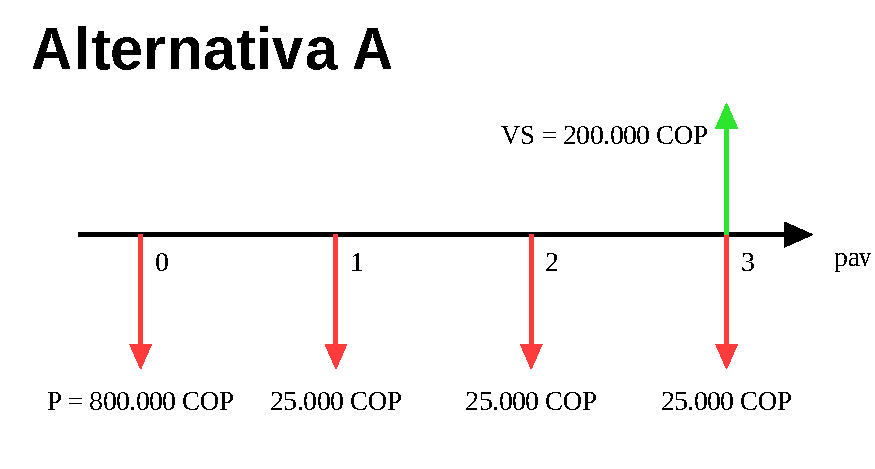
\includegraphics[trim=-5 -5 -5 -5, width=10.5cm, keepaspectratio]{10_Capitulo/img/ejemplos/PDFs/2/Ejemplo_2_A.pdf}}\\ \hline
		\multicolumn{3}{|c|}{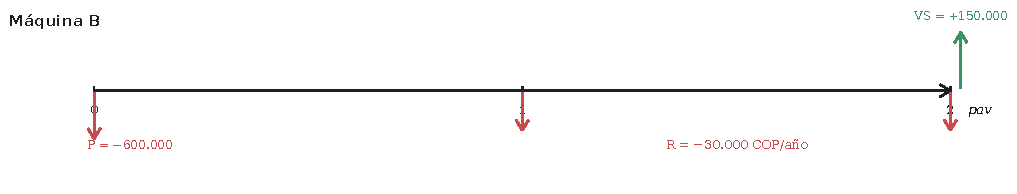
\includegraphics[trim=-5 -5 -5 -5, width=10.5cm, keepaspectratio]{10_Capitulo/img/ejemplos/PDFs/2/Ejemplo_2_B.pdf}}\\ \hline
		%%%%%%%%%%%%% FIN INSERCIÓN DE IMAGEN
		%%%%%FIN FLUJO DE CAJA

		%%%%% INICIO DECLARACIÓN FORMULAS
		%%%%%%%%%%% INICIO TITULO
		\rowcolor[HTML]{FFB183}
		\multicolumn{3}{|c|}{\cellcolor[HTML]{FFB183}\textbf{4. Declaración de fórmulas}} \\ \hline
		%%%%%%%%%%% FIN TITULO
  
		%%%%%%%%%%% INICIO MATEMÁTICAS
		\multicolumn{3}{|c|}{$VP=R\frac{1-(1+i)^{-n}}{i} \text{ Valor presente serie uniforme vencida}$}\\ 
		\multicolumn{3}{|c|}{$VF=R\frac{(1+i)^{n}-1}{i} \text{ Valor futuro serie uniforme vencida}$}\\
		\multicolumn{3}{|c|}{$CAUE = \sum \text{Ingresos}_{\text{anualizados}} - \sum \text{Egresos}_{\text{anualizados}} \text{ CAUE como sumatoria}$}\\
		\multicolumn{3}{|c|}{$A=P\frac{i}{1-(1+i)^{-n}} \text{ Recuperación de capital (serie uniforme vencida)}$}\\
		\multicolumn{3}{|c|}{$A=F\frac{i}{(1+i)^{n}-1} \text{ Fondo de amortización (serie uniforme vencida)}$}\\
		\hline
		%%%%%%%%%% FIN MATEMÁTICAS
  
		%%%%%% INICIO DESARROLLO MATEMÁTICO
		\rowcolor[HTML]{FFB183}
		%%%%%%%%%%INICIO TITULO
		\multicolumn{3}{|c|}{\cellcolor[HTML]{FFB183}\textbf{5. Desarrollo matemático}}   \\ \hline
		%%%%%%%%%% FIN TITULO
		%%%%%%%%%% INICIO MATEMÁTICAS
  
		Alternativa A & \multicolumn{2}{c|}{Alternativa B}\\ \hline

		\begin{tabular}[c]{@{}c@{}}Dividir los 800.000 COP \\ en 3 pagos anuales uniformes:\end{tabular} & \multicolumn{2}{c|}{\begin{tabular}[c]{@{}c@{}}Dividir los 600.000 COP \\ en 2 pagos anuales uniformes:\end{tabular}} \\
		$\begin{gathered}R_1 = 800{.}000\text{ COP}\mathbin{\color{red}\ast}\frac{0{,}36}{1-(1+0{,}36)^{-3}} \\ = 478{.}041{,}809\text{ COP}\end{gathered}$ & \multicolumn{2}{c|}{$\begin{gathered}R_1 = 600{.}000\text{ COP}\mathbin{\color{red}\ast}\frac{0{,}36}{1-(1+0{,}36)^{-2}} \\ = 470{.}237{,}288\text{ COP}\end{gathered}$}\\

        $ $  & \multicolumn{2}{c|}{}\\

        \begin{tabular}[c]{@{}c@{}}Dividir los 200.000 COP \\ en 3 pagos anuales uniformes:\end{tabular} & \multicolumn{2}{c|}{\begin{tabular}[c]{@{}c@{}}Dividir los 150.000 COP \\ en 2 pagos anuales uniformes:\end{tabular}} \\
		$\begin{gathered}R_2 = 200{.}000\text{ COP}\mathbin{\color{red}\ast}\frac{0{,}36}{(1+0{,}36)^{3}-1} \\ = 47{.}510{,}452\text{ COP}\end{gathered}$ & \multicolumn{2}{c|}{$\begin{gathered}R_2 = 150{.}000\text{ COP}\mathbin{\color{red}\ast}\frac{0{,}36}{(1+0{,}36)^{2}-1} \\ = 63{.}559{,}322\text{ COP}\end{gathered}$}\\

        $ $  & \multicolumn{2}{c|}{}\\

        $\begin{gathered}CAUE_{A} = -478{.}041{,}809\text{ COP} \\ - 25{.}000\text{ COP} + 47{.}510{,}452\text{ COP}\end{gathered}$ & \multicolumn{2}{c|}{$\begin{gathered}CAUE_{B} = -470{.}237{,}288\text{ COP} \\ - 30{.}000\text{ COP} + 63{.}559{,}322\text{ COP}\end{gathered}$}\\

        $ $  & \multicolumn{2}{c|}{}\\

        $CAUE_{A} = -455{.}531{,}357\text{ COP}$ & \multicolumn{2}{c|}{$CAUE_{B} = -436{.}677{,}966\text{ COP}$}\\

		\hline
		%%%%%%%%%% FIN MATEMÁTICAS
		%%%%%% FIN DESARROLLO MATEMÁTICO

		\rowcolor[HTML]{FFB183}
		\multicolumn{3}{|c|}{\cellcolor[HTML]{FFB183}\textbf{6. Respuesta}}    \\ \hline

		\multicolumn{3}{|c|}{La alternativa que representa menores pérdidas es la B.} \\ 
		\hline
	\end{longtable}
	%Se crean dos lineas en blanco para que no quede el siguiente texto tan pegado
	%\newline \newline
\end{center}
%%%%%%%%%%%%%%%%%%%%%%%%%%FIN EJERCICIO X %%%%%%%%%%%%%%%%%%%%%%%%%%%